\setcounter{chapter}{6}
\chapter{Campi Elettrici nei Mezzi Materiali}

\section{Dielettrici}

Nei capitoli precedenti si \`e introdotta la distinzione tra materiali \textit{conduttori} e \textit{isolanti}. Nella prima categoria definiamo tutte quelle sostanza che hanno un grande numero di elettroni liberi di muoversi all'interno della materia (per esempio i metalli); nel dettaglio vuol dire che ci sono elettroni che non sono legati a nessun nucleo (nei metalli il reticolo che definisce la struttura della materia \`e formato da ioni). 

Gli isolanti, vengono anche detti \textit{dielettrici} e a differenza dei precedenti la maggior parte delle cariche  hanno dei legami intensi con i nuclei del reticolo, di conseguenza l'unica cosa che possono fare \`e oscillare in modo limitato attorno all'atomo o molecola in presenza di campi elettrici esterni. Queste variazioni microscopiche causano effetti meno significativi rispetto ai conduttori dove si ha una completa riconfigurazione della distribuzione di carica, ma il sommarsi di questi scostamenti genera degli effetti apprezzabili all'interno del materiale.  


\subsection{Polarizzazione}

\begin{wrapfigure}{r}{0.4\textwidth}  % 'r' indica destra
    \centering
    \vspace{-1.2cm}
    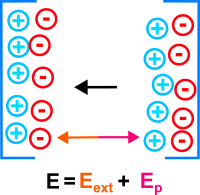
\includegraphics[width=4cm]{images/dieletrics}
\end{wrapfigure}
In presenza di un campo elettrico $\bold{E}_{ext}$ esterno i dielettrici hanno una ridistribuzione parziale delle cariche, tale fenomeno prende il nome di \textit{polarizzazione}. All'interno del materiale si instaura un campo elettrico di polarizzazione $\bold{E}_{p}$ con direzione opposta al campo elettrico a cui \`e sottoposto. 

Il campo complessivo che si sviluppa all'intero dell'isolante  ha la stessa direzione del campo esterno a cui \`e sottoposto.

\begin{equation}
	\bold{E} = \bold{E}_{ext} + \bold{E}_{p}
\end{equation} 
portando a una lieve riconfigurazione delle cariche. 

 All'interno del dielettrico \`e quindi presente un campo elettrico interno $\bold{E}_{int}$. Siccome le cariche non sono libere di muoversi essendo soggette a forze $\bold{F}_{mezzo}$ di natura atomica, all'interno del materiale si mantiene una condizione statica e di conseguenza la forza di Coulomb generata dal campo interno deve bilanciarsi:
\begin{equation}
	\bold{F} = \bold{F}_{mezzo} + q \bold{E}_{int} = 0
\end{equation}
Le forze d'interazione atomica sono di complessa determinazione e dipendono dalla configurazione atomica del materiale.  Dato che il campo interno \`e dato dall'espressione (7.1), si ha che noto il campo esterno per determinarne la sua espressione bisogna conoscere il campo di polarizzazione $\bold{E}_{p}$, ma il modo in cui si polarizzano le cariche e quindi $\bold{E}_{p}$ dipende da $\bold{E}_{int}$ e siccome (7.2) non \`e di facile risoluzione, abbiamo un problema circolare che non ci permette di determinare il valore del campo interno. Per calcolarlo \`e necessario passare da un altra strada.

In generale il mezzo \`e mediamente neutro e il campo di polarizzazione \`e nullo in assenza di un campo di stimolo, dovuto a sorgenti esterne.
\subsection{Costante Dielettrica Relativa}
Prima di dare una definizione matematica della polarizzazione, introduciamo una grandezza che caratterizza i materiali dielettrici, ottenuta dalle osservazione sperimentali di Faraday.

\begin{center}
	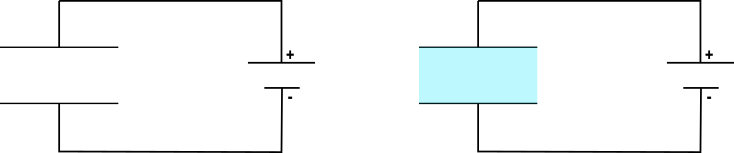
\includegraphics[width = 13cm]{images/faraday_exp}
\end{center}

Definiamo sperimentalmente un circuito formato da una sorgente di carica (batteria ideale) con una differenza di potenziale $\Delta \varphi$ e un condensatore planare. Sappiamo dai capitoli precedenti che la capacit\`a di un condensatore si lega alla carica e al potenziale nella relazione 
\begin{equation*}
	C = Q \Delta\varphi
\end{equation*}
Una volta misurata la capacit\`a del primo circuito si procede a realizzarne un secondo identico, in questo caso per\`o il condensatore viene riempito da un materiale dielettrico in tutto il volume compreso tra le armature. Affinch\`e la differenza di potenziale $\Delta \varphi$ resti la stessa deve cambiare la quantit\`a di carica che si distribuisce sulle superfici limite del condensatore, la identifichiamo con $Q'$.  

Di conseguenza si ha che $Q' > Q$ e di conseguenza di misura una capacit\`a $C' = Q' \Delta \varphi$ che risulta essere $C' > C$. Mettendo a confronto le due capacit\`a facendone il confronto troviamo che 
\begin{equation*}
	\frac{C'}{C} = \frac{Q'}{Q}
\end{equation*}
tale rapporto ci dice che il modo in cui cambia la capacit\`a del mezzo non dipende n\`e da $\Delta \varphi$ e nemmeno dalla geometria del condensatore, ma si ha una dipendenza solo dal mezzo dielettrico utilizzato.

Questo risultato ottenute per via empirica ci permette di introdurre una grandezza caratteristica dei dielettrici (come si discuter\`a pi\`u avanti, esistono diversi tipi di dielettrici e questa grandezza \`e caratteristica solo di quelli che risultano essere lineari e omogenei, ovvero il cui comportamento delle cariche \`e indipendente dalla direzione)
\begin{equation}
	\mathcal{E}_{r} = \frac{C'}{C}
\end{equation}
che prende il nome di \textbf{costante dielettrica relativa}.

\subsubsection{Interpretazione Fisica del Fenomeno}
\vspace{0.5cm}
\begin{center}
	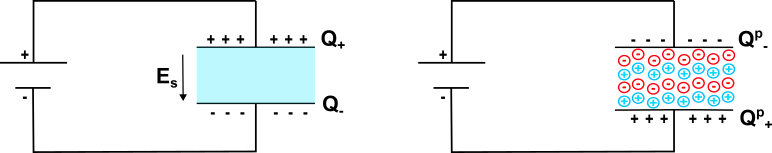
\includegraphics[width = 13cm]{images/faraday_exp1}
\end{center}

La differenza di potenziale ai capi del condensatore crea un campo elettrico di stimolo 
\begin{equation*}
	\bold{E}_s = \frac{Q'}{\varepsilon_0 A}\hat{u}_n
\end{equation*}
che sposta le cariche positive leggermente verso il basso e quelle negative verso l'alto (come nella seconda figura). Se prendiamo un elemento infinitesimo di volume del materiale tra le armature si ha che la distribuzione di carica resta neutra, ma se ci spostiamo verso le piastre del condensatore le cariche non si bilanciano e si ha una polarizzazione $\pm Q_{p}$. Questo eccesso di carica polarizzata sulle armature genera un campo di polarizzazione $\bold{E}_{p}$ con la stessa direzione di $\bold{E}_s$, ma verso opposto.

Per quanto definito nel paragrafo precedente il campo elettrico che osserviamo in laboratorio \`e dato da 
\begin{equation*}
	\bold{E} = \frac{Q'}{\varepsilon_0 A}\hat{u}_n + \bold{E}_p
\end{equation*}
dove 
\begin{equation*}
	\bold{E}_{p} \sim - \frac{Q_p}{\varepsilon_0 A}\hat{u}_n
\end{equation*}

\subsubsection{Analogia con un conduttore inserito tra le armature}

\vspace{0.5cm}
\begin{center}
	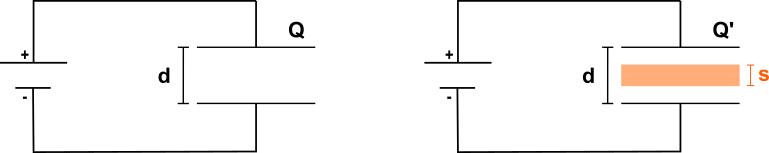
\includegraphics[width = 13cm]{images/faraday_conduct}
\end{center}
Se prendiamo l'integrale 
\begin{equation*}
	\Delta \varphi = \int_0^d \bold{E} \cdot d\bold{s} 
\end{equation*}
per una configurazione in cui tra le due armature \`e presente il vuoto si deve avere che $\Delta \varphi = Qd/\varepsilon_0 A $, mentre in quella in cui \`e presente il dielettrico $\Delta \varphi = Q'd/\varepsilon_0 A + E_p d$ ; affinch\`e le due cadute di tensione siano le medesime abbiamo bisogno che $\bold{E}_p < 0$ e $Q' > Q$. Quindi la carica nel mezzo si deve spostare affinch\`e si abbia un eccesso sulle superfici. 
\newline


Questo risultato \`e analogo a quello che si \`e ottenuto nel capitolo sull'elettrostatica; se ipotizziamo di inserire tra le armature del condensatore un conduttore di spessore $s < d $ e vogliamo mantenere una differenza di potenziale $\Delta \varphi$ costante, osserveremo una riorganizzazione delle cariche sulle piastre con carica $Q'$.

\begin{wrapfigure}{r}{0.4\textwidth} % 'r' for right, 'l' for left, width of figure
    \centering
    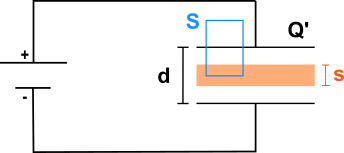
\includegraphics[width=0.38\textwidth]{images/faraday_conduct1} % Adjust width accordingly
\end{wrapfigure}
Tale conseguenza \`e facilmente dimostrabile considerando un circuito S, che abbraccia sia la parte interna del conduttore che quella esterna al condensatore (come in figura), e calcolandone il flusso del campo elettrico attraverso.
\begin{equation*}
	\phi_S(\bold{E}) = 0
\end{equation*}
e quindi possiamo concludere che internamente non \`e presente carica $Q_{int} = 0$. Dato che internamente non \`e possibile avere della carica questa deve per forza essere distribuita sulle superfici limite del conduttore e del condensatore, infatti sul conduttore si ha che $Q_{ind} = - Q'$. Nelle regioni  interne al condensatore in cui non \`e presente il conduttore si misura in modulo un campo elettrostatico
\begin{equation*}
	E_1 = E_2 = \frac{Q'}{\varepsilon_0 A} \frac{d -s}{2}
\end{equation*} 
e quindi una differenza di potenziale 
\begin{equation*}
	\Delta \varphi = \int_0^d \bold{E} \cdot d \bold{s} = \frac{Q'}{\varepsilon_0A}(d-s)
\end{equation*}
Confrontando la carica $Q'$ con quella $Q$ nel caso in cui tra le armature sia presente il vuoto si ha che 
\begin{equation*}
	Q' = Q \frac{d}{d-s} > Q
\end{equation*}
Da questa dimostrazione, possiamo vedere come l'esperimento con un conduttore sia un caso limite per  di un dielettrico in cui la carica di polarizzazione indotta coincide con la carica esterna. Se espandiamo il conduttore in tutto lo spazio del condensatore (come con il dielettrico), $s \to d$, abbiamo che la carica $Q' \to \infty$ e usando la definizione di costante dielettrica relativa si ha che $\mathcal{E}_r \to \infty$. 

Un ulteriore informazione che possiamo ottenere da questa analogia \`e la distinzione tra che cosa \`e un conduttore e che cosa \`e un dielettrico (isolante), definiamo dunque:
\begin{enumerate}
	\item \textit{conduttore}, tutti quei mezzi per cui $\mathcal{E}_r \to \infty$ e per cui si ha induzione totale $Q_{ind} = - Q'$;
	\item \textit{dielettrico}, tutti quei mezzi per cui $1 < \mathcal{E} < \infty$ e si ha una polarizzazione delle cariche dove $|Q_p| < |Q'|$
\end{enumerate}

Dato che $ Q'> Q$ si ha che $Q'/Q > 1$ e quindi possiamo concludere che $\mathcal{E}_r > 1$ ha un limite inferiore. La variabilit\`a della costante dielettrica dipende dalle propriet\`a microscopiche atomiche e molecolari di cui \`e composto il mezzo. 
\newline

La descrizione macroscopica che abbiamo dato del fenomeno \`e comune a tutti i materiale ed \`e sempre riconducibile all'interpretazione in termini di polarizzazione, ovvero
\begin{enumerate}
	\item le cariche non sono libere (non possono essere rimosse toccando un mezzo polarizzato con un conduttore, al contrario di questi ultimi);
	\item il mezzo ha una distribuzione di carica positiva e negativi con "baricentri" differenti, anche se rimane globalmente neutro.
\end{enumerate}

\begin{remark}
Nei prossimi capitoli vedremo come per campi variabili che cambiano rapidamente lo spostamento delle cariche di polarizzazione pu\`o non essere necessariamente in fase con il campo elettrico.	
\end{remark}

\section{Sviluppo in Multipoli del Potenziale Elettrostatico}

\begin{wrapfigure}{r}{0.4\textwidth} % 'r' for right, 'l' for left
    \centering
    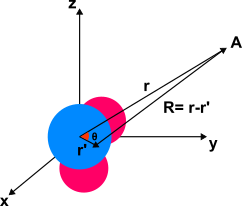
\includegraphics[width=0.38\textwidth]{images/multipolo} % Adjust width
\end{wrapfigure}

Diamo una descrizione generale del campo elettrico dovuto ad una distribuzione di carica $\rho = \rho(\bold{r})$. Consideriamo un volume infinitesimo $d \nu$ identificato dal vettore posizione $\bold{r}'$ e calcoliamo il potenziale in un punto A nello spazio esterno alla distribuzione, posto a una distanza $\bold{r}$ dal sistema di riferimento.

Possiamo esprimere $\bold{R}$, il vettore che identifica la posizione del volume rispetto al punto A, in funzione di $\bold{r}$ e $\bold{r'}$. Per farlo usiamo la legge dei coseni considerando un angolo $\theta$ compreso tra $\bold{r}$ e $\bold{r'}$:
\begin{equation}
	R = \sqrt{r^2 + r'^2 - 2rr'\cos\theta}
\end{equation} 
L'espressione del potenziale nel punto A \`e data da 
\begin{equation*}
	\varphi_A = \frac{1}{4 \pi \varepsilon_0} \int_{V} \frac{\rho (\bold{r}')}{R}d\nu'
\end{equation*}
e sostituendo (7.4) al suo interno si ha 
\begin{equation}
	\varphi_A = \int_{V} \rho \;d \nu' \,[r^2 + r'^2 - 2rr'\cos\theta]^{-1/2}
\end{equation}
Siamo interessati al caso in cui $r \gg r'$, un caso concreto \`e quando vogliamo misurare il campo macroscopico a grande distanza, dovuto alla distribuzione di carica di atomi o molecole.

Riscriviamo (7.4) raccogliendo rispetto a $r^2$
\begin{equation*}
	R = r\left[1 + \left( \frac{r'^2}{r^2}\right) -2\,\frac{r'}{r}\,\cos\theta\right]^{1/2}
\end{equation*}
per le condizioni definite possiamo pensare ad R come a una funzione 
\begin{equation*}
	R = [1 + \varepsilon]^{1/2} \quad \varepsilon \to 0
\end{equation*}
e quindi possiamo sviluppare con Taylor al secondo ordine rispetto alla variabile $\varepsilon = \left( \frac{r'^2}{r^2}\right) -2\,\frac{r'}{r}\,\cos\theta$
\begin{equation*}
	\frac{1}{R} \simeq \frac{1}{r} \left(1 - \frac{1}{2} \varepsilon + \frac{3}{8}\varepsilon^2 + \dots\right) = \frac{1}{r} \left[ 1 + \frac{r'}{r}\cos \theta + \left(\frac{r'}{r}\right)^2  \frac{3 \cos\theta -1}{2} + \mathcal{O}\left(\frac{r'}{r}\right)^3\right]
\end{equation*}
Dato che $r$ non dipende dalla variabile d'integrazione, sostituendo lo sviluppo in (7.5) troviamo 
\begin{align}
	 \varphi_A & \simeq \frac{1}{4 \pi \varepsilon_0} \left[ \frac{1}{r} \int_{V} \rho(\bold{r}')d\nu' + \frac{1}{r^2} \int_{V} r' \cos\theta \rho(\bold{r}')d \nu' + \dots \right] = \notag \\ \rule{0pt}{30pt} 
	 & =  \frac{1}{4 \pi \varepsilon_0} \left[ \frac{k_0}{r} + \frac{k_1}{r^2} + \frac{k_2}{r^3}+ \dots \right] 
\end{align}
dove con $k_0,k_1,k_2, ecc \dots$, abbiamo indicato gli integrali corrispettivi alla potenza di $r$. Per proseguire con lo sviluppo prendiamo quanto segue come postulato senza verificarlo:

\begin{center}
\fbox{\parbox{12cm}{\textit{Il potenziale in un punto lontano $r \gg r'$ qualasiasi \`e determinato dal primo termine non nullo dello sviluppo di multipolo.}}}	
\end{center}

Il primo termine dello sviluppo prende il nome di \textbf{momento di monopolo}:
\begin{equation}
	K_0 = \int_{V} \rho(\bold{r}') d \nu' = Q_0
\end{equation}
dove $Q_0$ \`e la carica netta delle distribuzioni, ovvero corrisponde al potenziale di una carica puntiforme. Se abbiamo la stessa quantit\`a di cariche positive e negative, come nel caso delle molecole neutre, $K_0$ sar\`a nullo. 

\begin{remark}
Dal postulato definito, possiamo assumere che per distanze grandi il termine $K_0$ prevariva su tutti gli altri termine dello sviluppo e quindi il campo elettrico sar\`a quello di una carica puntiforme.	
\end{remark}

Il secondo termine \`e chiamato \textbf{momento di dipolo elettrico}:
\begin{equation}
	K_1 = \int_{V} r' \cos\theta \rho (\bold{r}') d \nu'	
\end{equation}
poich\`e $r' \cos \theta = z'$, questo termine misura lo spostamento relativo delle cariche verso A. Se $K_0 = 0$, il termine $K_1$ \`e dominante e questo avviene nel caso di un materiale dielettrico neutro e polarizzato.

\subsection{Potenziale di Dipolo}

Siccome siamo interessati ai materiali dielettrici possiamo tranquillamente porre $K_0 = 0$ e concentrarci sullo studio di $K_1$. Osserviamo che il termine $r' \cos\theta $ \`e la proiezione di $r'$ lungo la direzione del vettore $\bold{r}$ e possiamo riscriverlo come 
\begin{equation*}
	\bold{r'} \cos \theta = \bold{r}' \cdot \hat{u}_{r}
\end{equation*}
sostituendo in $K_1$ si ha che il potenziale arrestato al primo ordine nello sviluppo di multipolo diventa 
\begin{equation}
	\varphi_{A} =  \frac{\hat{u}_{r}}{r^2} \cdot \int_{V} \bold{r}' \rho(\bold{r}) d \nu' 
\end{equation}
Il secondo termine del prodotto scalare coincide con un vettore le cui dimensioni sono quelle di una carica per una lunghezza. Questo vettore viene indicato con il termine $\bold{p}$:
\begin{equation}
	\bold{p} = \int_{V} \bold{r}' \rho(\bold{r}) d\nu'
\end{equation} 
e usando questa espressione possiamo riscrivere l'equazione (7.9) come:
\begin{equation}
	\varphi_{A}(\bold{r}) = \frac{\hat{u}_{r} \cdot \bold{p}}{r^2}
\end{equation}
Il termine di dipolo di una distribuzione di carica \`e completamente determinato da $\bold{p}$. Di conseguenza il potenziale \`e il campo elettrico sono equivalenti a quello di una coppia di cariche uguali ed opposte, separate da una distanza $\bm{\delta}$.

\subsubsection{Esempio}

Consideriamo due cariche puntiformi $q^{\pm } = \pm q$ rispettivamente individuate da un raggio vettore $\bold{r}_{\pm}$ uscente dall'origine di un sistema di riferimento; la distanza tra di esse \`e data da $\bm{k} = \bold{r}_{+} - \bold{r}_{-}$. Utilizzando la funzione $\delta$ di Dirac ( che ricordiamo non essere realmente una funzione, ma una distribuzione), definiamo la distribuzione di carica nel seguente modo
\begin{equation*}
	\rho_{\pm}(\bold{r}) = \pm q \delta(\bold{r} - \bold{r}_{\pm})
\end{equation*}  
esprimendo la nostra assenza d'informazione sul modo in cui \`e fatta la distribuzione di carica di un punto. Il momento di dipolo associato \`e dato da 
\begin{equation*}
	\bold{p} = \int_{V} q \delta(\bold{r}- \bold{r}_{+})d\bold{r} - \int_{V} q \delta(\bold{r}-\bold{r}_{-})d\bold{r} = q(\bold{r}_{+} - \bold{r}_{-})
\end{equation*}

Per calcolare il dipolo di una distribuzione neutra \`e sufficiente conoscere la carica positiva e negativa totale e la separazione tra il centro di carica delle distribuzioni e quindi studiare il campo di una distribuzione neutra usando la relazione (7.11) e il fatto che $\bold{E} = - \nabla \varphi$. 

Usando le coordinate sferiche troviamo che 
\begin{align*}
\left \{ \begin{array}{l}
	\bold{E}_{r} = - \frac{\partial \varphi}{\partial r} \hat{u}_{r} = \frac{2p \cos\theta}{4 \pi \varepsilon_0 r^3} \hat{u}_{r} \\ \rule{0pt}{20pt}
	\bold{E}_{\theta} = \frac{1}{r} \frac{\partial \varphi}{\partial \theta}\hat{u}_{\theta} = \frac{p \sin \theta}{4 \pi \varepsilon_0 r^3}\hat{u}_{\theta}
\end{array}\right.
\end{align*}
Il campo elettrico lontano dal dipolo ($r \gg \delta)$ decresce come $\bold{E} \sim 1/r^3$. 

\begin{remark}
\
\begin{enumerate}
	\item Il campo di un dielettrico polarizzato \`e dato dalla sovrapposizione di campi di dipolo
	\item Nella nostra descrizione di dipolo magnetico per un mezzo dielettrico abbiamo dato una descrizione macroscopica del fenomeno, ci rimane da descrivere come il comportamento dei dipoli elementari determini la polarizzazione del mezzo che si osserva macroscopicamente.
\end{enumerate}	
\end{remark}

\section{Azione Meccanica di un Campo Elettrico su un Dipolo }
\subsection{Campo Elettrico Uniforme}
Supponiamo che $+q$ e $-q$ siano due cariche tenute insieme meccanicamente in modo tale che la loro distanza $\delta$ resti costante (un esempio sono le molecole polari), sfruttiamo l'equivalenza $\bold{p} = q \bm{\delta}$ per descrivere l'interazione del dipolo con un campo elettrostatico $\bold{E}$ uniforme.
\begin{center}
\fbox{\parbox{15cm}{
\begin{remark}
Ad una distribuzione di carica  ridotta ad una coppia di cariche $\pm q$ separate da una distanza $\bm{\delta} $ corrisponde un solo momento di dipolo $\bold{p}$; ad un dipolo $\bold{p}$ corrisponde un numero infinito di rappresentazioni $\bold{p} = q \bm{\delta}$. Ogni risultato pu\`o dipendere solo dal prodotto $q \bm{\delta}$ e non da $q$ e $\bm{\delta}$ separatamente.	
\end{remark}
}}
\end{center}
\begin{center}
	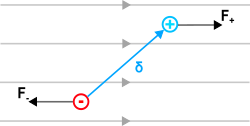
\includegraphics[width = 7cm]{images/fieldaction}
\end{center}

Su ciascuna carica del dipolo agisce una forza di Coulomb $\bold{F}_{\pm} = \pm q \bold{E}$, con stessa direzione, ma verso opposto. Dando un descrizione della fisica dal centro di massa del dipolo si ha che la risultante delle forze agenti \`e nulla
\begin{equation*}
	\bold{F}_{cm} = \bold{F}_{+} + \bold{F}_{-} = 0
\end{equation*}
Anche se questa risulta essere uguale a zero \`e presente un momento della forza che agisce sul sistema e lo mette in rotazione. Posti come bracci delle rispettive forze i vettori posizione $\bold{r}_{+}$ e $\bold{r}_{-}$ con origine nel centro di massa (come in figura) si ha che il momento torcente totale \`e dato dall'equazione :

\begin{center}
	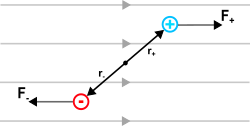
\includegraphics{images/forcemoment}
\end{center}

\begin{equation*}
	\bm{\tau} = \bold{r}_{+} \times \bold{F}_+ + \bold{r}_{-} \times \bold{F}_{-} = (\bold{r}_+ - \bold{r}_-) \times q\bold{E} = q \bm{\delta} \times \bold{E}
\end{equation*}
e quindi possiamo riassumere $\bm{\tau}$ come:
\begin{equation}
	\bm{\tau} = \bold{p} \times \bold{E}
\end{equation} 
il cui valore \`e indipendente dalla scelta del polo. 

Il momento della forza esercitato sul dipolo rigido risulta essere nullo quando questi si allineano nella direzione campo elettrico, dando luogo al fenomeno della \textit{polarizzazione}.
\begin{center}
\fbox{\parbox{15cm}{
\begin{remark}
Notare che in generale il campo $\bold{E}$ considerato per definire (7.12) \`e il campo risultante dalla somme di tutte le cariche presenti nel sistema: distribuzione esterna e altri dipoli	
\end{remark}
}}
\end{center}

\subsubsection{Energia Potenziale}

L'orientamento del dipolo in cui il momento $\bold{p}$ \`e parallelo al campo elettrico $\bold{E}$ corrisponde alla configurazione in cui l'energia \`e al livello pi\`u basso; se vogliamo cambiarne la disposizione dobbiamo compiere del lavoro contro il campo elettrico. Ipotizziamo di voler ruotare il dipolo di un angolo $\theta_0$, considerando il contributo dato dal lavoro rispetto alla carica positiva si ha
\begin{equation*}
\Delta U_{\pm} = - \int_0^{\Delta s} \bold{F}_{\pm} \cdot d\bold{s} = qE \, \frac{\delta}{2}\,(1- \cos \theta)
\end{equation*}
dove $\Delta s = \delta/2(1-\cos\theta)$. Il lavoro complessivo tenendo conto anche della carica negativa \`e infinite dato da 
\begin{equation*}
	\Delta U = \Delta U_+ + \Delta U_- = 2 \Delta U_+ = q \delta E(1-\cos\theta) = pE(1-\cos \theta)
\end{equation*}
In modo del tutto analogo, possiamo ricavare il lavoro rispetto al momento della forza agente sul dipolo:
\begin{equation*}
	\Delta U = - \int_0^{\theta_0} \tau d\theta  = - \int_0^{\theta_0} pE \sin\theta d\theta = pE(1-\cos \theta_0)
\end{equation*}
Poich\`e l'energia potenziale \`e definita a meno di una costante, possiamo esprimerla come 
\begin{equation}
	U = -pE \cos\theta = - \bold{p} \cdot \bold{E}
\end{equation} 
dove questa assume valore minimo quando $\bold{p}$ \`e parallela a $\bold{E}$ e massimo quando $\bold{p}$ \`e antiparallela al campo elettrico.

\begin{center}
	\fbox{\parbox{15cm}{
	\begin{remark}
		 Per un dipolo rigido non si ha bisogno di altri contributi all'energia potenziale definita in (7.13), per vederlo possiamo vedere i termini 
			\begin{equation*}
				U_{\pm} = \mp\int_{\infty}^{r_+} q \bold{E} \cdot d\bold{s} = - dW_{\pm} 
			\end{equation*}
			 al lavoro necessario per portare le cariche $\pm q$ da $\infty $ ad una distanza $r_{\pm}$ dal centro di massa del dipolo. Inoltre dobbiamo tenere conto dell'energia d'interazione  tra le cariche portate ad una distanza relativa $\delta$: 
			 \begin{equation*}
			 	U_{+-} = \frac{q^2}{4 \pi \varepsilon_0} \frac{1}{\delta} 
			 \end{equation*}
	Complessivamente la configurazione ha un energia potenziale 
	\begin{equation*}
		U = - \int_\infty^{r_+}q \bold{E} \cdot d\bold{s} + \int_{\infty}^{r_-} q\bold{E} \cdot d \bold{s} +  \frac{q^2}{4 \pi \varepsilon_0} \frac{1}{\delta}
	\end{equation*}
Il termine $U_{+-}$ \`e l'energia di configurazione del dipolo (auto-energia), questa dipende da $q$ e $\delta$ separatamente, esiste anche se campo elettrico $\bold{E}$ esterno \`e nullo ed infine per un dipolo rigido questa risulta essere costante; proprio per quest'ultima propriet\`a possiamo considerarlo come un termine trascurabile e quindi scrivere l'energia come in (7.13). 
	\end{remark}
	}}
\end{center} 

Se il dipolo risulta avere una distanza non tra le cariche variabile si ha che $\bold{p} \sim \bold{E}$ e l'energia potenziale \`e data da 
\begin{equation}
	U = - \frac{1}{2} \bold{p} \cdot \bold{E}
\end{equation}

\subsection{Dipolo Non Rigido Soggetto ad un Campo Elettrico Non Uniforme}

Se il campo elettrico $\bold{E}$ non \`e uniforme, come per esempio quello di una carica puntiforme, dato un dipolo privo di vincoli di rigidit\`a, si ha che le cariche costituenti vengono tirate dall'intensit\`a del campo e all'interno dell'espressione dell'energia potenziale compare un termine d'interazione tra le cariche. 

Per dimostrarlo osserviamo che la forza  totale agente sul dipolo \`e non nulla rispetto al caso in cui il campo $\bold{E}$ era uniforme 
\begin{equation*}
	\bold{F} = q [\bold{E}(\bold{r}_+) - \bold{E}(\bold{r}_{-})] = q \Delta \bold{E}
\end{equation*}
dove $\Delta \bold{E}$ \`e la variazione del campo elettrico sulla distanza $\bm{\delta} = (\bold{r}_+ - \bold{r}_-)$. Per ciascuna coordinata cartesiana, la variazione pu\`o essere espressa tramite il differenziale:
\begin{align*}
	\Delta E_{x} = \frac{\partial E_x}{\partial x} \Delta x + \frac{\partial E_x}{\partial y} \Delta y + \frac{\partial E_x}{\partial z}\Delta z = \nabla E_x \cdot \bm{\delta} \\ \rule{0pt}{30pt} 
	\Delta E_{y} = \frac{\partial E_y}{\partial x} \Delta x + \frac{\partial E_y}{\partial y} \Delta y + \frac{\partial E_y}{\partial z}\Delta z = \nabla E_y \cdot \bm{\delta} \\ \rule{0pt}{30pt}
		\Delta E_{z} = \frac{\partial E_z}{\partial x} \Delta x + \frac{\partial E_z}{\partial y} \Delta y + \frac{\partial E_z}{\partial z}\Delta z = \nabla E_z \cdot \bm{\delta} \\ 
\end{align*}
e di conseguenza ciascuna componente della forza \`e esprimibile come 
\begin{align}
\left \{ \begin{array}{l}
\bold{F}_{x} = \bold{p} \cdot \nabla E_x \\ \rule{0pt}{20pt}
\bold{F}_{y} = \bold{p} \cdot \nabla E_y \\ \rule{0pt}{20pt}
\bold{F}_{z} = \bold{p} \cdot \nabla E_z
\end{array}\right.
\iff \bold{F} = (\bold{p} \cdot \nabla )\,\bold{E} 	
\end{align}
La forma compatta espressa a destra \`e una scrittura simbolica che raggruppa tre relazioni scalari per le componenti.

\subsubsection{Esempio}

Consideriamo un dipolo che interagisce con una carica puntiforme di un qualsiasi segno; poich\`e i dipoli tendono ad allinearsi al campo elettrico, il momento di dipolo e il gradiente di $\nabla E$ sono discordi in verso e di conseguenza si ha che la forza tra un dipolo e una carica puntiforme \`e sempre attrattiva a prescindere dal segno.

\section{Polarizzazione dei Mezzi}

L'interazione delle cariche legate di un mezzo con un campo elettrico $\bold{E}$ ne determinano la sua polarizzazione. A livello atomico o molecolare compare un dipolo $\langle \bold{p} \rangle $ proporzionale al campo stesso.

Sperimentalmente possiamo osservare due tipologie di mezzi:

\begin{enumerate}
	\item polari: avviene per orientamento delle molecole, che per natura hanno dei baricentri di carica non allineati e sono dotate di un momento di dipolo elettrico elementare;
	\item apolari: sono la maggior parte dei mezzi e la polarizzazione avviene per deformazione atomica.
\end{enumerate}

\subsection{Mezzi Polari}
\begin{wrapfigure}{r}{0.4\textwidth} % 'r' for right, 'l' for left
    \centering
    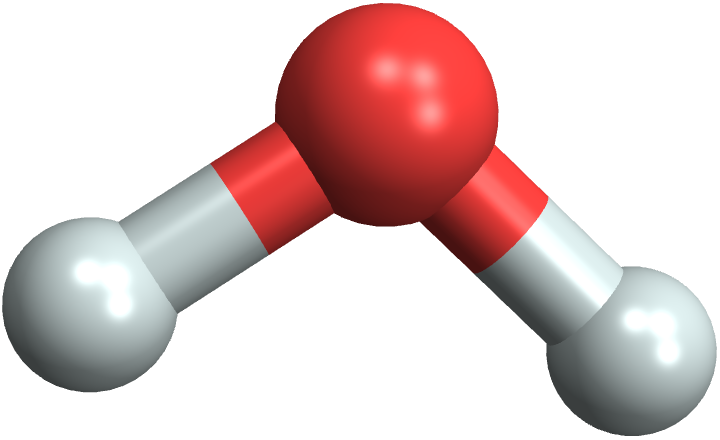
\includegraphics[width=0.38\textwidth]{images/water} % Adjust width
\end{wrapfigure}
Un esempio di mezzo polare \`e dato dall'acqua le cui molecole $\bm{H_2O}$ presentano un asimmetria di carica, generando un momento di dipolo permanente (rigido) dell'ordine di $\bold{p_0} \sim 6.1 \times 10^{-30}$.  

In assenza di un campo elettrico $\bold{E}$, all'interno della materia le molecole (e quindi il momento di dipolo) hanno un orientazione casuale e quindi il valore medio del momento in volume \`e $\langle \bold{p} \rangle = 0$. Nel caso in cui compaia un campo elettrico $\bold{E}_{ext}$ di stimolo all'esterno del mezzo, si ha un loro allineamento parziale contrastato dall'agitazione termica, che per un dato volume porta ad avere un momento di dipolo medio $\langle \bold{p} \rangle $ proporzionale al campo elettrico complessivo $\bold{E}$.
\newline

Per esempio se consideriamo un campo elettrico $\bold{E}  = 10^6 \frac{V}{m}$, il lavoro necessario ad orientare le cariche da ortogonali a parallele \`e dato da 
\begin{equation*}
	\Delta U_{max} = 2p_0 E \simeq 10^{-23} \,J \simeq 10^{-4} \,eV \simeq 0,1\, meV
\end{equation*}
L'agitazione termina per un volume d'acqua a temperatura ambiente \`e data da $k_B T \sim 25 meV$. Dunque si ha che il lavoro necessario ad orientare le cariche \`e 1/100 dell'energia termica nel sistema, questo vuol dire che i dipoli subiscono una variazione minima, ma che statisticamente per la loro moltitudine diventa significativa. Infatti il momento di dipolo medio ortogonale \`e $\langle \bold{p}_{\bot} \rangle = 0 $, mentre quello parallelo al campo \`e $\langle \bold{p} \rangle = p_0 \langle \cos \theta \rangle \neq 0$, ottenendo cos\`i un allineamento parziale.

Se in un volume consideriamo $n_0$ molecole e di queste $n_i$ hanno un certo momento di dipolo $p_i$ con angolo $\theta_i$, il momento di dipolo medio \`e dato da 
\begin{equation*}
	\langle p \rangle = \frac{1}{n_0} \sum_i n_i\,p_i = \frac{1}{n_0} \sum_i n_i \,p_0\cos\theta_i
\end{equation*} 
che nel limite al continuo assume l'espressione
\begin{equation}
	\langle p \rangle = \frac{1}{n_0} \int n(\theta) p_0 \cos \theta d \Omega 
\end{equation}
Utilizzando la teoria cinetica dei gas (meccanica statica classica), la distribuzione di probabilit\`a di trovare una molecola tra energia $U$ e $U+dU$ \`e data dalla distribuzione di Boltzmann:
\begin{equation*}
	n = n_0 e^{-U/k_bT}
\end{equation*}
Dati che l'energia per singolo dipolo $U_i \ll kT$ dell'energia termica, possiamo esprimere il fattore di
Boltzmann in serie di Taylor al primo ordine 
\begin{equation*}
	e^{-U/k_B T} \sim 1 + \frac{p_0 E \cos\theta}{k_b T}
\end{equation*}
L'equazione (7.16) esprimendo l'angolo solido $d \Omega = 2 \pi \sin\theta d\theta$ e sostituendo al suo interno lo sviluppo, risulta essere proporzionale a 
\begin{equation*}
	\langle p \rangle \;\alpha \; \frac{p_0^2}{k_b T} E
\end{equation*}
questo ci dice che la polarizzazione media \`e proporzionale al campo elettrico (mezzo lineare)

\begin{center}
\fbox{\parbox{15cm}{
\begin{remark}
Se il campo elettrico \`e molto intenso ( $\gg 10 ^9 \, V/m$) e si \`e a bassa temperature affinch\`e $k_b T \leq U$, l'orientamento dei dipoli pu\`o diventare completo. In questo limite il comportamento non \`e lineare e $\langle p \rangle$ raggiunge un valore di saturazione. 	
\end{remark}
}}
\end{center}

\subsection{Polarizzazione Atomica: Dipoli Indotti}

La polarizzazione per deformazione \`e presente in tutti i mezzi (anche polari) ed \`e associata al fatto che ogni atomo \`e rappresentabile come una distribuzione di cariche negative (elettroni) al cui centro \`e presenta della carica positiva (nucleo).

\begin{center}
	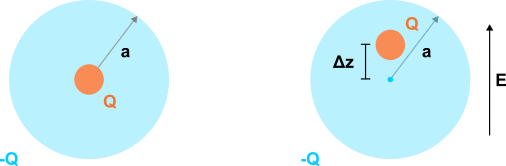
\includegraphics{images/distribuzione}
\end{center}
Introducendo un campo elettrico esterno $\bold{E}$ la carica positiva si sposta di un tratto $\Delta z$ rispetto al centro della distribuzione di carica negativa, in questo modo. viene a formarsi un momento di dipolo elettrico
\begin{equation*}
	p = Q \Delta z
\end{equation*}
Il protone raggiunge una condizione di equilibrio quando la risultante delle forze diventa nulla 
\begin{equation*}
	\bold{F}_{p} = q^+ \bold{E} + q^+ \bold{E}_{el} = 0
\end{equation*}
dove $\bold{E}_{el}$ \`e il campo interno dovuta alla distribuzione di carica dell'elettrone, che in prima approssimazione possiamo assumere sferica. Il modulo del campo elettrico dato dalla nube elettronica \`e calcolabile usando la legge di Gauss:
\begin{equation*}
	E_{el}(\Delta z) 4 \pi (\Delta z)^2 = \frac{4}{3}\pi (\Delta z)^3 \frac{\rho}{\varepsilon_0} \quad \Rightarrow  \quad E_{el}(\Delta z) = \frac{p}{4 \pi \varepsilon_0} \frac{1}{a^3}
\end{equation*}
dove $a$ \`e il raggio atomico e $a  = 1 \,\AA $. Infinite dalla condizione di equilibrio deduciamo che campo elettrico di stimolo e campo interno coincidono in modulo e quindi la polarizzazione si lega al campo esterno come 
\begin{equation}
	\bold{p} = 4 \pi \varepsilon_0 a^3 \bold{E}
\end{equation}
Questo modello primitivo fornisce una stima corretta dell'ordine di grandezza della polarizzabilit\`a atomica:
\begin{equation}
	\bold{p} = \alpha \bold{E}
\end{equation}
dove il fattore $\alpha $ prende il nome di \textbf{polarizzabilit\`a}.

Le polarizzazioni atomiche sono deboli, ma misurabili; questo \`e dovuto al fatto che i momenti di dipolo sono tutti paralleli e in macro regioni sono presenti grandi quntit\`a di atomi o molecole.

Fino a questo punto abbiamo dato una descrizione della polarizzazione di un singolo atomo e quindi non del mezzo intero che ne \`e costituito; per fornire una descrizione macroscopica del fenomeno, partendo dai risultati microscopici, introduciamo una grandezza vettoriale di polarizzazione 
\begin{equation}
	\bold{P}  = \mathcal{N} \bold{p}
\end{equation}
dove il termine $\mathcal{N}$ rappresenta la densit\`a di dipoli per unit\`a di volume, mentre $\bold{p}$ \`e il momento di dipolo elementare. $\bold{P}$ prende il nome di \textbf{vettore di polarizzazione}  e rappresenta il momento di dipolo per unit\`a di volume. Dimensionalmente coincide con la densit\`a di carica superficiale:
\begin{equation*}
	[P] = \frac{C}{m^2}
\end{equation*}
Ad ogni volume elementare $d \tau $ del mezzo possiamo associare un momento di dipolo 
\begin{equation*}
	\bold{p}_{\tau} = \bold{P} d \tau
\end{equation*}
\begin{wrapfigure}{r}{0.4\textwidth} % 'r' for right, 'l' for left
    \centering
    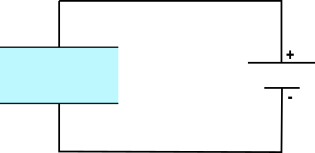
\includegraphics[width=0.38\textwidth]{images/dielRC} % Adjust width
\end{wrapfigure}
Usando questa informazione immaginiamo di assemblare una lastra uniforme di materiale dielettrico polarizzato e di volerne calcolare il campo elettrico $\bold{E}$ che osserviamo nel sistema del laboratorio se la colleghiamo ad un alimentatore.   Dai paragrafi precedenti sappiamo che il campo elettrico complessivo \`e dato da 
\begin{equation*}
	\bold{E} = \bold{E}_{s} + \bold{E}_{p}
\end{equation*}
dove $\bold{E}_{s}$ \`e il campo elettrico di stimolo ottenuto nel caso in cui tra le piastre del condensatore \`e presente il vuoto. Dato che $\bold{E}_{s}$ \`e uniforme e $\bold{P} = \alpha \bold{E}$ anche la polarizzazione \`e uniforme nel mezzo. Per calcolare il campo $\bold{E}_p$ in un punto $A$ esterno al dielettrico, definiamo un cilindro tra le due armature la cui area della base \`e $da$ e ne isoliamo un volume con altezza $dz$.

\begin{center}
	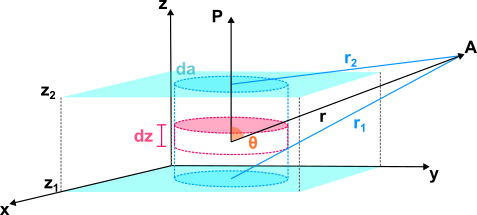
\includegraphics[width = 10cm]{images/polfield}
\end{center}
Siccome conosciamo l'espressione del potenziale elettrico nel punto A in funzione di un dipolo elettrico elementare, possiamo calcolare 
\begin{equation}
	d \varphi_{A} = \frac{\bold{p}_{\tau} \cdot \hat{u}_{r}}{ 4 \pi \varepsilon_0 r^2} = \frac{P\,\text{da}\, \text{dz} \cos \theta }{4 \pi \varepsilon_0 r^2}
\end{equation}

\begin{wrapfigure}{r}{0.4\textwidth} % 'r' for right, 'l' for left
    \centering
    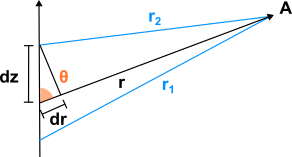
\includegraphics[width=0.38\textwidth]{images/anglerel} % Adjust width
\end{wrapfigure}
Integrando rispetto alla variabile $z$  l'equazione  (7.20) diventa 
\begin{equation*}
	d \varphi_{A} = \frac{Pda}{4 \pi \varepsilon_0} \int_{z_1}^{z_2} \frac{dz \cos\theta}{r^2}
\end{equation*}
usando la relazione $dz = - dr \cos\theta$ esprimiamo l'integrale rispetto alla coordinata radiale $r$:
\begin{equation}
	d \varphi_{A} = - \frac{Pda}{4 \pi \varepsilon_0} \int_{r_1}^{r2} \frac{dr}{r^2} = \frac{Pda}{4 \pi \varepsilon_0} \left(\frac{1}{r_2} - \frac{1}{r_1}\right)
\end{equation}
Il termine $Q_P^{\pm} = \pm Pda$ \`e equivalente alla carica di polarizzazione sulla superficie superiore o inferiore della colonna. Estendendo all'intera superficie, il potenziale \`e equivalente a quello generato da una distribuzione superficiale doppia di carica con densit\`a $\sigma_{P} = \pm P$.

\begin{center}
	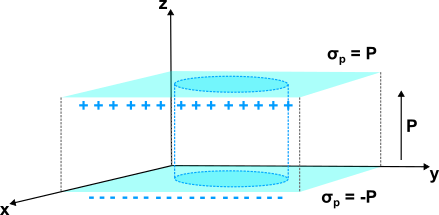
\includegraphics[width = 10cm]{images/distpol}
\end{center}
All'interno  di ciascuna colonna i dipoli elementari $ \bold{p} = \bold{P} d\tau$ hanno cariche uguali e contrarie sulle superfici opposte del cilindro. Internamente la carica nel  mezzo \`e neutro e rimane solo il contributo al campo sulla superficie esterna. Di conseguenza abbiamo un campo elettrico all'interno del materiale, che possiamo assumere essere dipendente da una distribuzione di carica superficiale di polarizzazione e utilizzare gli strumenti dell'elettrostatica per calcolarlo. Utilizzando la legge di Gauss per una configurazione di carica data da due armature parallele, tra cui \`e presente il vuoto,  abbiamo che il campo interno \`e dato da
\begin{equation*}
	\bold{E}_{void} = \frac{\sigma_{P}}{\varepsilon_0} \hat{u}_{n}
\end{equation*}
e quindi il potenziale associato alle due piastra poste a distanza $d$ \`e pari a 
\begin{equation}
	\Delta \varphi_{AB} = \int_{A}^{B} \bold{E}_{void} \cdot d\bold{s} = \frac{\sigma_{P}}{\varepsilon_0} d = \frac{P}{\varepsilon_0}d
\end{equation}
Potremmo domandarci se l'equazione (7.22) sia corretta, ovvero che  non esista un cammino particolare che unisca i punti A e B delle rispettive armature, per cui si misuri una differenza di potenziale differente. Se consideriamo un cammino esterno come in figura tra i punti $A$ e $B$
\begin{center}
	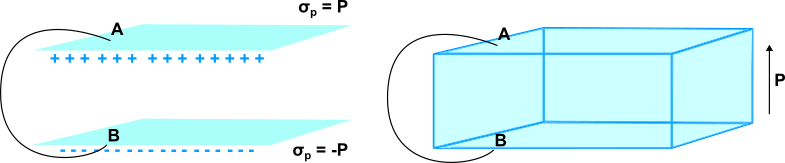
\includegraphics[width = 15cm]{images/dielpath}
\end{center}  

siccome il campo elettrico esterno \`e il medesimo anche la differenza di potenziale \`e la medesima. Diverso \`e il discorso per il campo elettrico all'interno, dato che la lastra \`e composta da milioni di atomi con campi diretti in modo del tutto casuale;  siccome per\`o il campo elettrico \`e una grandezza conservativa $\nabla \cdot \bold{E} = 0$, presi due punti A e B con un cammino passante all'interno del materiale, si deve avere lo stesso valore di $\Delta \varphi_{AB}$ qualsiasi questo sia.
\begin{center}
	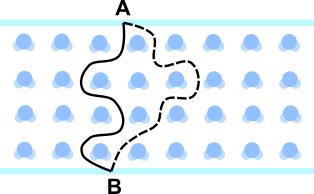
\includegraphics{images/doublepath}
\end{center}
Sia che si scelga un percorso interno o esterno, la differenza di potenziale misurata \`e sempre la stessa data da (7.22), di conseguenza per un mezzo polarizzato la differenza di potenziale all'interno del mezzo \`e 
\begin{equation*}
	\Delta \varphi_{AB} = \int_{A}^{B} \bold{E}_p \cdot d\bold{s} = \frac{P}{\varepsilon_0}d
\end{equation*}
Localmente il campo elettrico non \`e uniforme dato che cambia in base alla distanza a cui ci si trova dal campo prodotto da atomi e/o molecole, ma se consideriamo il campo medio su un volume, questo \`e pari a 
\begin{equation}
	\langle \bold{E}_p \rangle  = \frac{1}{V} \int_{V} \bold{E}_p \cdot d\bm{\tau} = - \frac{\bold{P}}{\varepsilon_0}
\end{equation}
Il campo complessivo sar\`a dato dalla relazione 
\begin{equation*}
	\bold{E} = \bold{E}_{s} + \bold{E}_p = \frac{\Delta \varphi}{d} - \frac{\bold{P}}{\varepsilon_0}
\end{equation*}

Siccome $\bold{P}$ dipende da $\Delta \varphi$ e per conoscere $\Delta \varphi$ devo prima aver calcolato $\bold{P}$, il problema \`e circolare. Per calcolare il vettore di polarizzazione $\bold{P}$ abbiamo due strategie, una \`e quella di conoscere densit\`a del materiale e valore dei dipoli elementari per ricostruirlo e la seconda \`e la sua misurazione per via macroscopica. Nel secondo caso per determinarlo confrontiamo la configurazione rispetto al vuoto con quella in cui \`e presente un mezzo dielettrico, come nel caso delle osservazioni empiriche di Faraday.

\begin{center}
	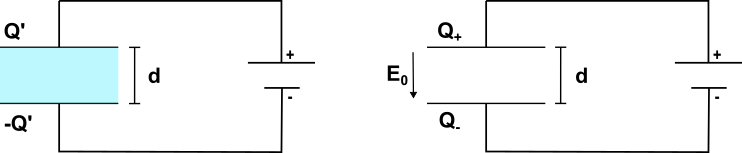
\includegraphics[width = 12cm]{images/faraday_exp2}
\end{center} 
Possiamo porre $\bold{P}$ in relazione a $\bold{E}$ tramite la relazione fenomenologica $Q = \varepsilon_r Q_0$ dove $Q_0$ \`e la carica che corrisponde ad un condensatore con la stessa geometria del dielettrico, ma nel vuoto e a parti\`a di potenziale $\varphi_{12}$.
 
 Nel configurazione con il dielettrico e senza il campo \`e dato da 
 \begin{equation*}
 	E = \frac{\Delta \varphi_{12}}{d} = \frac{Q'}{\varepsilon_0A} - \frac{\bold{P}}{\varepsilon_0} \quad \text{e} \quad E_0 = \frac{\Delta \varphi_{12}}{d}  = \frac{Q_0}{\varepsilon_0 A}
 \end{equation*} 
 il cui primo elemento in possiamo riscrivere come
 \begin{equation*}
 	E = \frac{\varepsilon_{r}Q_0}{\varepsilon_0 A} - \frac{P}{\varepsilon_0} = \varepsilon_r E_0 - \frac{P}{\varepsilon_0}
 \end{equation*}
 dato che $E = E_0$ possiamo ricavare il vettore potenziale in funzione del campo $\bold{E}$
 \begin{equation}
 	\bold{P} = \varepsilon_0(\varepsilon_r -1) \bold{E} = \varepsilon_0 \chi_{E} \bold{E}
 \end{equation}
 dove il termine $\chi_{E} = \varepsilon_{r}-1$ prende il nome di \textbf{suscettivit\`a elettrica} di un mezzo.  Il vettore macroscopico di polarizzazione \`e legato al campo elettrico da un fattore empirico $\varepsilon_{r}$ che \`e possibile misurare in un sistema a due piatti paralleli e che caratterizza il mezzo.
 
 Mettendo in relazione le due espressioni che abbiamo dato di $\bold{P}$ troviamo un secondo modo con cui esprimere $\chi_{E}$:
 \begin{equation*}
 	\mathcal{N} \bold{p} =\mathcal{N} \alpha \bold{E} = \varepsilon_0 \chi_{E} \bold{E}
 \end{equation*}
 e segue che 
 \begin{equation}
 	\chi_{E} = \frac{\alpha \mathcal{N}}{\varepsilon_0}
 \end{equation}
 collegando cos\`i grandezze microscopiche con quelle macroscopiche. 
 
 \begin{center}
 \fbox{\parbox{15cm}{
 	\begin{remark}
 	\
 	\begin{enumerate}
 		\item Il campo $\bold{E}  = - \bold{P} /\varepsilon_0$ \`e specifico della geometria che si \`e considerata, vale per alcune geometrie notevoli, ma non per tutte.
 		\item $\bold{P} = \varepsilon_0 \chi_{E} \bold{E}$ vale per mezzi isotropi e lineari; in casi pi\`u generali $\chi_{E} = \chi_{E}(\bold{E})$  e possono esserci anche fenomeni di anisotropia.
 	\end{enumerate}
 	\end{remark} 	
}}
 \end{center}

\section{Relazione Generale tra il Campo di Polarizzazione e il Vettore di Polarizzazione}
Consideriamo un dielettrico con una polarizzazione qualsiasi e una qualsiasi geometria.
\begin{wrapfigure}{l}{0.4\textwidth} % 'r' for right, 'l' for left
    \centering
    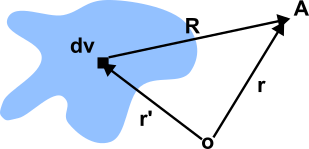
\includegraphics[width=0.38\textwidth]{images/poldistro} % Adjust width
\end{wrapfigure}
Per un volume infinitesimo $d \nu$  il potenziale nel punto A per un dipolo \'e:
\begin{equation*}
	d \varphi_{A} = \frac{1}{4 \pi \varepsilon_0} \frac{d \bold{p} \cdot \hat{u}_{R}}{R^2} = \frac{1}{4 \pi \varepsilon_0} \frac{\bold{P} \cdot \hat{u}_{R}}{R^2}d\nu
\end{equation*}
Integrando sul volume del dielettrico
\begin{equation}
	\varphi_{A} = \frac{1}{4 \pi \varepsilon_0} \int_{V} \frac{\bold{P} \cdot \hat{u}_{R}}{R^2}d \nu
\end{equation}

\begin{center}
	\fbox{\parbox{15cm}{
	\begin{remark}
		\
		\begin{enumerate}
			\item l'espressione \`e vero anche per A all'interno del volume del dielettrico, intesa come media su un volume microscopicamente grande e macroscopicamente piccolo;
			\item lo sviluppo in multipoli richiede che $ r \gg r' $: condizione che risulta essere macroscopicamente vera dappertutto, eccetto nel volume $d\nu$ per il dipolo $d\bold{p} = \bold{P} d\nu$, ma queste non \`e rilevante in quanto un dipolo non interagisce con se stesso.
		\end{enumerate}
	\end{remark}
	}}
\end{center}
L'espressione (7.26) \`e completa, ma il significato \`e pi\`u chiaro se rendiamo leggibile il legame con le cariche di polarizzazione, a tal fine usiamo l'identit\`a 
\begin{equation*}
	\nabla' \left (\frac{1}{R}\right) = \frac{\hat{u}_{R}}{R^2}
\end{equation*}
e la propriet\`a della divergenza di un vettore per uno scalare:
\begin{equation*}
	\nabla' \left( \frac{\bold{P}}{R}\right) = \bold{P} \cdot \nabla' \left(\frac{1}{R} \right) + \frac{\nabla' \cdot \bold{P}}{R}
\end{equation*}
Sostituendo in (7.26) l'espressione diventa 
\begin{align*}
	\varphi_{A} & = \frac{1}{4 \pi \varepsilon_0} \int_{V} \frac{\bold{P} \cdot \hat{u}_{R}}{R^2} d \nu = \frac{1}{4 \pi \varepsilon_0} \int_{V} \bold{P} \cdot \nabla' \left( \frac{1}{R}\right)d\nu = \\ \rule{0pt}{30pt}
	& = \frac{1}{4 \pi \varepsilon_0} \int_{V} \nabla ' \cdot \left( \frac{\bold{P}}{R}\right)d\nu - \frac{1}{4 \pi \varepsilon_0} \int_{V} \frac{\nabla' \cdot \bold{P}}{R}d \nu
\end{align*}
Utilizzando il teorema di Gauss (o della divergenza) il primo termine pu\`o essere tradotto in un integrale di superficie:
\begin{equation}
	\varphi_{A} = \frac{1}{4 \pi \varepsilon_0} \int_{S} \frac{\bold{P} \cdot d\bold{a}}{R} - \frac{1}{4 \pi \varepsilon_0} \int_{V} \frac{\nabla' \cdot \bold{P}}{R}d \nu
\end{equation}
Il primo termine \`e identificabile come il potenziale di una distribuzione superficiale di carica con densit\`a 
\begin{equation}
	\sigma_{p} \equiv \bold{P} \cdot \hat{\bold{n}} 
\end{equation}
mentre il secondo termine \`e il potenziale di una distribuzione volumica di carica con densit\`a:
\begin{equation}
	\rho_{p} \equiv - \nabla \cdot \bold{P}
\end{equation}
con queste definizioni l'equazione (7.27) diventa:
\begin{equation}
	\varphi_{A} = \frac{1}{4 \pi \varepsilon_0} \int_{S} \frac{\sigma_{p} da}{|\bold{r} - \bold{r}'|} + \frac{1}{4 \pi \varepsilon_0} \int_{V} \frac{\rho_{p} d \nu}{|\bold{r} - \bold{r}'|}
\end{equation}

\subsubsection{Esempio 1}
Una lastra di dielettrico con polarizzazione uniforme, abbiamo visto che pu\`o essere come due armature in parallelo sui cui \`e presente una densit\`a di carica superficiale $\sigma_{P} = \pm P$, sulla superficie laterale $\sigma_{P} = 0$ poich\`e $\bold{P} \cdot d \bold{a} $. Inoltre la densit\`a di volume \`e $\rho_{P} = - \nabla \cdot \bold{P} = 0$ dato che la polarizzazione \`e uniforme.
\newpage 

\subsubsection{Esempio 2 : Sfera uniformemente polarizzata}

\begin{wrapfigure}{l}{0.4\textwidth} % 'r' for right, 'l' for left
    \centering
    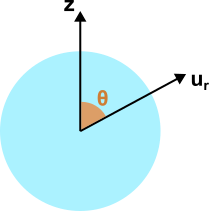
\includegraphics[width=0.38\textwidth]{images/dielsphere} % Adjust width
\end{wrapfigure}

Per dielettrico di forma sferica e uniformemente polarizzato abbiamo che la densit\`a di carica sulla superficie non \`e uniforme, infatti
\begin{equation*}
	\sigma_{P} = \bold{P} \cdot \hat{u}_{r} = P\cos\theta
\end{equation*}
In generale $\sigma_{P}$ \`e uniforme se $\bold{P}$ risponde alla geometria del sistema. Inoltre $\rho_{p} = 0$, in configurazioni simmetriche in cui $\rho =0$ nel mezzo.

Possiamo delineare le seguenti casistiche per quando la densit\`a di volume di un dielettrico \`e nulla:
\begin{equation*}
	\rho_{p} = \nabla \cdot \bold{P}  = 0 \iff \bold{P} \; \alpha \; \left \{ \begin{array}{l}
		\text{uniforme in coordinate cartesiane} \\ \rule{0pt}{15pt} 
		 \frac{\hat{u}_{r}}{r} \; \text{in coordinate cilindriche } \\ \rule{0pt}{15pt}
		 \frac{\hat{u}_{r}}{r^2} \; \text{coordinate sferiche}
	\end{array}\right.
\end{equation*}

In un dielettrico la carica legata \`e nulla (dielettrico neutro) e la carica in ogni porzione di volume \`e il flusso di $- \bold{P}$:
\begin{equation*}
	Q_{p}^{V} = \int_{V} \rho_{p} d \nu = - \int_{V} \nabla' \cdot \bold{P} d \nu = - \int_{S} \bold{P} \cdot d \bold{a} = - \int_{S} \sigma_{p} da = - Q_{p}^{S}
\end{equation*}

\section{Legge di Gauss (per i Dielettrici)}

Il flusso del campo elettrico $\bold{E}$ dipende dalla carica totale netta racchiusa da una superficie. Nel caso dei dielettrici possiamo utilizzare la legge di Gauss aggiungeno un termine in pi\`u che tiene conto delle cariche di polarizzazione:
\begin{equation*}
	\int_{S} \bold{E} \cdot d\bold{a} = \frac{1}{\varepsilon_0} \int_{V} (\rho + \rho_{p}) d \nu
\end{equation*}
e in form a differenziale 
\begin{equation*}
	\nabla \cdot \bold{E} = \frac{1}{\varepsilon_0} ( \rho + \rho_{p})
\end{equation*}
Siccome $\rho_p$ non \`e nota a priori, ma dipende da $\bold{E}$, conviene riformulare l'espressione rispetto alla polarizzazione usando la relazione $\rho_{p} = - \nabla \cdot \bold{P}$ in questo modo:
\begin{equation*}
	\nabla \cdot (\varepsilon_0 \bold{E} + \bold{P}) = \rho
\end{equation*}
Definiamo la grandezza vettoriale:
\begin{equation}
	\bold{D} = \varepsilon_0 \bold{E} + \bold{P}
\end{equation}
che prende il nome di \textbf{vettore di induzione elettrica} (o campo elettrico ausiliario). Per un mezzo dielettrico la legge di Gauss pu\`o essere riformulata assume la forma 
\begin{equation}
	\nabla \cdot \bold{D} = \rho
\end{equation}
La divergenza di $\bold{D}$ dipende solo dalle cariche libere presenti nel mezzo ( che possiamo vedere come le sorgenti del campo di stimolo).

\subsection{Relazione Costitutiva}

La legge di Gauss (7.32) non \`e sufficiente per il risolvere il problema dell'elettrostatica in forma completa. Per ricavare $\bold{E}$, $\bold{P}$, $\sigma_p$ e $\rho_p$, \`e necessario conoscere la relazione empirica:
\begin{equation*}
	\bold{D} = \bold{D}(\bold{E})
\end{equation*}
detta \textbf{relazione costitutiva}.

In mezzi omogenei e lineari, abbiamo tradotto la relazione empirica come 
\begin{equation*}
	\varepsilon_{r} = \frac{C'}{C}
\end{equation*}
nella relazione tra vettore di polarizzazione e campo elettrico:
\begin{equation*}
	\bold{P} = \varepsilon_0 \chi_{E} \bold{E} \quad \text{dove} \quad \chi_{E} = \varepsilon_{r} -1
\end{equation*}
Dunque (7.31) si traduce in 
\begin{equation*}
	\bold{D} = \varepsilon_0 \bold{E} + \bold{P} = \varepsilon_0 \varepsilon_r \bold{E} \equiv \varepsilon \bold{E}
\end{equation*}
dove $\varepsilon$ prende il nome di \textbf{costante dielettrica del mezzo}.

\subsection{Equazione di Maxwell per L'elettrostatica}
Tenendo conto di quanto definito per i mezzi dielettrici, abbiamo bisogno di aggiustare anche le equazioni di Maxwell affinch\`e queste ne descrivano il comportamento, le prime due leggi assumono l'espressione 
\begin{equation*}
	\left \{ \begin{array}{l}
		\nabla \cdot \bold{D} = \rho \quad (I)\\ \rule{0pt}{15pt}
		\nabla \times \bold{E} = 0 \quad [- \partial \bold{B} / \partial t] \quad (II)
	\end{array} \right.
\end{equation*}
L'equazione di Faraday (II) non contiene sorgenti e non \`e modificata dalla presenza di carica di polarizzazione. In mezzi omogenei e lineari 
\begin{equation*}
	\nabla \times \bold{D} = \nabla \times (\varepsilon_0 \varepsilon_r \bold{E}) = \varepsilon_0 \varepsilon_r \nabla \times \bold{E} = 0
\end{equation*}
In generale per\`o $\bold{D} = \bold{D}(\bold{E})$ pu\`o non essere lineare 
\begin{equation*}
	\nabla \times \bold{D} = \nabla \times (\varepsilon_0 \bold{E} + \bold{P})
\end{equation*}
pu\`o essere diverso da zero, dato che $\bold{P}$ pu\`o non essere conservativo.

\subsection{Relazione di continuit\`a per $\bold{E}$ e $\bold{D}$}

\begin{wrapfigure}{l}{0.4\textwidth} % 'r' for right, 'l' for left
    \centering
    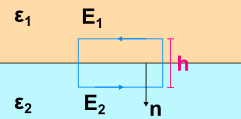
\includegraphics[width=0.38\textwidth]{images/nounidiel} % Adjust width
\end{wrapfigure}
Consideriamo un mezzo costituito da due materiali dielettrici differenti con costante dielettrica del mezzo $\varepsilon_1$ e $\varepsilon_2$. All'interfaccia tra i due dielettrici in presenza di campo elettrico esiste della carica superficiale di polarizzazione anche in assenza di cariche libere. Ipotizzando che la carica libera nel mezzo $\rho = 0$, utilizziamo le equazioni di Maxwell per determinare come i campi si legano tra loro sulla superficie interna ed esterna.

Siccome i campi elettrici sono conservativi deve valere che 
\begin{equation*}
	\int_{\Gamma} \bold{E} \cdot d\bold{s} = 0
\end{equation*}

facendo tendere $h \to 0 $ si ha che 
\begin{equation*}
	E_{1}^{//} = E_{2}^{//}
\end{equation*}
\begin{wrapfigure}{r}{0.4\textwidth} % 'r' for right, 'l' for left
    \centering
    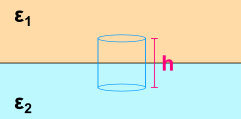
\includegraphics[width=0.38\textwidth]{images/nounidiel1} % Adjust width
\end{wrapfigure}
e quindi la componente del campo elettrico sulla superficie non ha discontinuit\`a. 

Ricorrendo alla legge di Gauss $\nabla \cdot \bold{D} = 0$, e prendendo una superficie cilindrica che attraversa l'interfaccia del mezzo, si ha che per $h \to 0 $:
\begin{equation*}
	\int_{S} \bold{D} \cdot d\bold{a} = 0 \Rightarrow (\bold{D}_{1} - \bold{D}_2) \cdot \bold{n} = 0
\end{equation*}
che equivale alla condizione
\begin{equation*}
	\varepsilon_1 E_{1,\bot} = \varepsilon_2 E_{2,\bot}
\end{equation*}
La componente ortogonale di $\bold{D}$ non ha discontinuit\`a, ma il campo elettrico con direzione ortogonale \`e discontinuo, infatti
\begin{equation*}
	\Delta E_{\bot} = \frac{\Delta P}{\varepsilon_0} \quad \iff \quad \Delta E_{\bot} = \frac{\sigma_{p,1}-\sigma_{p,2}}{\varepsilon_0}
\end{equation*}

\begin{wrapfigure}{l}{0.4\textwidth} % 'r' for right, 'l' for left
    \centering
    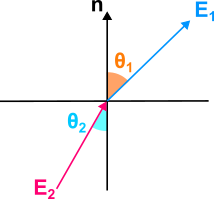
\includegraphics[width=0.38\textwidth]{images/incident} % Adjust width
\end{wrapfigure}
ed \`e dovuto alla presenza di una distribuzione di carica di polarizzazione $\sigma_{p} \neq 0$ lungo la superficie condivisa dai due materiali. Riassumendo il campo elettrico nel mezzo si comporta come 
\begin{equation*}
	\left \{ \begin{array}{l}
	E_{1,//} = E_{2,//} \\ \rule{0pt}{20pt}
	E_{1, \bot} = \frac{\varepsilon_2}{\varepsilon_1}E_{2, \bot}	
	\end{array}\right.
\end{equation*} 


Possiamo riscrivere le due componenti del campo in coordinate polari, definendo l'angolo d'incidenza rispetto alla normale della superficie limite:
\begin{equation*}
	\left \{ \begin{array}{l}
		E_1 \sin \theta_1 = E_2 \sin \theta_2 \\ \rule{0pt}{20pt}
		\varepsilon_1 E_1 \cos \theta_1 = \varepsilon_2 E_2 \cos\theta_2
	\end{array}\right.
\end{equation*}
 Da queste relazioni abbiamo che 
 \begin{equation*}
 	\tan(\theta_1) = \frac{\varepsilon_2}{\varepsilon_1} \tan(\theta_2)
 \end{equation*}
 Se si hanno mezzi con costanti dielettriche differenti, i campi elettrici all'interno del mezzo cambiano direzione.
 
\subsection{Problemi di Elettrostatica con i Dielettrici}

Possiamo determinare due categorie di problemi e un loro approccio risolutivo:
\newline

	1) Mezzi continui e lineari con medesima simmetria (planare, cilindrica o sferica) delle sorgenti e dielettrico.

\subsubsection{Esempi}

\begin{center}
	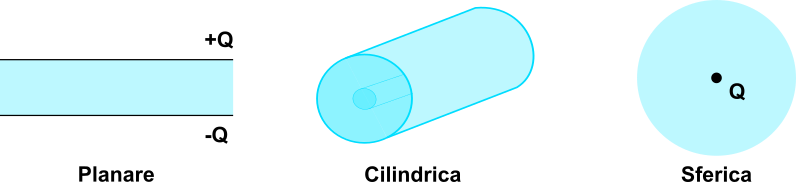
\includegraphics[width = 15cm]{images/configuration}
\end{center}	
In questi casi il problema \`e facilmente risolubile, usando la legge di Gauss per $\bold{D}$ su una superficie opportuna (dove $\bold{D}$  \`e costante), e una volta trovato $\bold{D}$ il resto segue a cascata.

Le relazioni tra i campi sono indipendenti dalla specifica simmetria 
\begin{equation*}
	\left \{ \begin{array}{l}
		\bold{E} = \frac{\bold{D} }{\varepsilon_0 \varepsilon_r} \\ \rule{0pt}{20pt}
		\bold{P} = \varepsilon_0(\varepsilon_{r} -1) \bold{E} = \frac{\varepsilon_{r} -1 }{\varepsilon_r} \bold{D}
	\end{array}\right.
\end{equation*}
Per queste geometrie vale che :
\begin{itemize}
	\item I campi $\bold{E}, \bold{D}$ e $\bold{P}$ sono sempre paralleli in un mezzo omogeneo e lineare;
	\item Tutti i campi coinvolti ($\bold{E}, \bold{D}, \bold{P}$ e $\bold{E}_s,\bold{E}_p$) e le distribuzioni $\sigma_{p}$ e $\rho_{p}$ seguono la simmetria del mezzo;
	\item La relazione tra $\bold{E}$ e $\bold{E}_{s}$ (campo di stimolo dovute alle sorgenti libere nel vuoto) e tra $\bold{P}$ e $\bold{E}_{p}$ (campo delle sorgenti di polarizzazione) sono indipendenti dalla geometria:
	\begin{align*}
	\left \{ \begin{array}{l}
		\bold{E} = \frac{\bold{E}_{s}}{\varepsilon_r} \\ \rule{0pt}{20pt}
		 \bold{E}_p = \bold{E} - \bold{E}_s = - \frac{\bold{P}}{\varepsilon_0}
	\end{array}\right.
	\end{align*}
\end{itemize}

\begin{center}
	\fbox{\parbox{15cm}{
	\begin{remark}
		In generale quanto discusso non \`e vero per geometrie pi\`u complesse.
	\end{remark}
	}}
\end{center}

\subsubsection{Esempio}

Consideriamo un dielettrico a simmetria sferica, lineare e omogeneo attorno a una carica Q posta nel suo centro. Per determinarne il campo elettrico prodotto, possiamo pensare di applicare la stessa strategia utilizzata da Faraday per determinare empiricamente $\varepsilon_{r}$. Decomponiamo la configurazione presercando la simmetria in una in cui \`e presente solo la sorgente di cariche libere e una in cui \`e presente solo la sorgente di carica polarizzata.

\begin{center}
	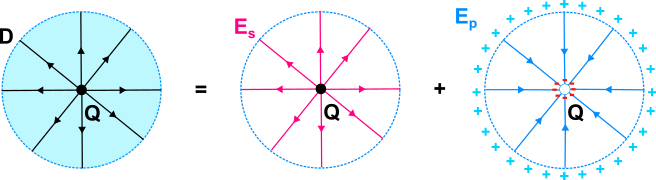
\includegraphics[width = 15cm]{images/spheredecomp}
\end{center}
Il problema per calcolare $\bold{E}_s$ ha la stessa simmetria del problema per $\bold{D}$. Risolviamo per $\bold{D}$ usando la legge di Gauss per una superficie a $r$ fissato.
\begin{equation*}
	D(r) 4 \pi r^2 = Q \quad \Rightarrow  \quad \bold{D}(r) = \frac{Q}{4 \pi r^2} \hat{u}_{r}
\end{equation*}
da cui calcoliamo il campo elettrico
\begin{equation*}
	\bold{E} = \frac{Q}{4 \pi \varepsilon_0 \varepsilon_{r}} \frac{\hat{u}_r}{r^2}
\end{equation*}
Il campo di stimolo nel vuoto coincide con quello prodotto da una carica puntiforme 
\begin{equation*}
	\bold{E}_{s}(r) = \frac{Q}{4 \pi \varepsilon_0} \frac{\hat{u}_{r}}{r^2}
\end{equation*}
e quindi possiamo riscrivere il campo elettrico totale come 
\begin{equation*}
	\bold{E} = \frac{1}{\varepsilon_{r}} \bold{E}_{s} \quad \text{per } r < R
\end{equation*}
e quindi l'intensit\`a del campo e della forza esercitata \`e ridotto di un fattore $\varepsilon_{r}$ all'interno del mezzo materiale. Questo genera una discontinuit\`a del campo quando si passa da dentro al mezzo all'esterno dove si ipotizza esserci il vuoto.
\begin{equation*}
	\Delta E_{r} = \frac{Q}{4 \pi \varepsilon_0} \frac{1}{r^2} - \frac{Q}{4 \pi \varepsilon_0\varepsilon_{r}} \frac{1}{r^2} = \frac{Q}{4 \pi \varepsilon_0} \frac{1}{r^2} \left(\frac{\varepsilon_r -1}{\varepsilon_r}\right)
\end{equation*}
Vettore e campo di polarizzazione sono dunque dati da:
\begin{equation*}
	\left \{ \begin{array}{l}
		\bold{P} = \varepsilon_0 \chi_{E} \bold{E} = \frac{Q}{4 \pi} \left(\frac{\varepsilon_r -1 }{\varepsilon_r}\right)\frac{\hat{u}_{r}}{r^2} \\ \rule{0pt}{20pt}
		\bold{E}_{p} = \bold{E} - \bold{E}_{s} = \frac{Q }{4 \pi \varepsilon_0}\left(\frac{1}{\varepsilon_r} -1\right) = - \frac{\bold{P}}{\varepsilon_{0}}
	\end{array}\right.
\end{equation*}
Conoscendo il vettore $\bold{P}$ possiamo ora calcolare la distribuzione di carica di polarizzazione:

\begin{equation*}
	\sigma_P = \pm \bold{P} \cdot \hat{n} = P(r) 
\end{equation*}
per una superficie sferica, inoltre 
\begin{equation*}
	\rho_{p} = - \nabla \cdot \bold{P} = - \frac{1}{r^2} \frac{\partial^2 }{\partial r^2}\left(r^2 P_{r}\right) = 0
\end{equation*} 
La carica totale di polarizzazione sulla superficie del mezzo \`e data da 
\begin{equation*}
	Q_{p}^{s} = \int_{S} \bold{P} \cdot d \bold{a} = \int_{S} \frac{Q}{4 \pi }\left(\frac{\varepsilon_r -1}{\varepsilon_r}\right) \frac{\hat{u}_{r}}{r^2} \cdot r^2\sin\theta d\theta d\varphi \,\hat{u}_{r} = \left(\frac{\varepsilon_r -1 }{\varepsilon_r} \right)Q
\end{equation*}
Notare come nel caso limite in cui $\varepsilon_{r} \to \infty$ (conduttore), si ha $Q_{p}^{s} = Q$ ossia induzione totale.
\newline

Se la superficie limite del dielettrico non \`e sferica, $\sigma_p$ non \`e uniforme, ma 
\begin{equation*}
	Q_{p}^{s} = \left(\frac{\varepsilon_r -1 }{\varepsilon_r} \right)Q
\end{equation*}
dato che $Q_{p}^{s} = \phi_{S}(\bold{P})$ e $P(r) \; \alpha \; 1/r^2$. Inoltre se la carica libera non \`e uniformemente distribuita nel dielettrico $\rho = \rho (\bold{r})$ si ha che la distribuzione di carica polarizzata nel dielettrico $\rho_p \neq 0$.
\newline

2) Per configurazioni senza simmetrie, e/o che possiedono interfacce si ha che le cariche di polarizzazione non hanno in generale la simmetria del campo di stimolo $\bold{E}_{s}$, inoltre sia $\bold{E}_{p}$ e $\bold{E}_{s}$ non sono paralleli tra loro e il campo elettrico di polarizzazione $\bold{E}_{p}$ non risponde alla simmetria delle sorgenti.

Per determinare gli opportuni campi si pu\`o ricorre a condizioni al contorno e di raccordo all'interfaccia tra i mezzi per trovare $\sigma_{p}$ e $\rho_{p}$ e formulare il problema in termini di problema generale dell'elettrostatica.

\subsection{Caso Notevole: Campo di una Sfera Dielettrica con $\bold{P}$ uniforme}
\begin{wrapfigure}{l}{0.4\textwidth} % 'r' for right, 'l' for left
    \centering
    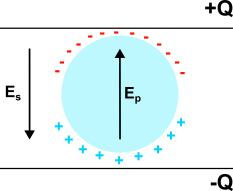
\includegraphics[width=0.38\textwidth]{images/spherepol} % Adjust width
\end{wrapfigure}

In generale la polarizzazione che si forma in dielettrico \`e uniforme se il campo esterno (ovvero quello di stimolo) \`e uniforme, il che avviene solo per geoemetrie ellisoidali. Di cui un dielettrico a simmetria planare, cilindrica o sferica sono i casi limite.

Se anzich\`e avere una sfera di materiale dielettrico come in figura, avessimo un sfera conduttrice  internamente il campo elettrico sarebbe nullo, ovvero il campo d'induzione \`e uguale ed opposto a quello esterno $\bold{E}_{s}$. Siccome questa configurazione \`e esprimibile come caso limite per un dielettrico possiamo immaginarci per continuit\`a che per un dielettrico isotropo e lineare si sviluppi al suo interno un campo di polarizzazione $\bold{E}_{p}$ antiparallelo ad $\bold{E}_{s}$.

Il campo $\bold{E}_{p}$ deve essere uniforme in quanto va a compensazione di un campo a sua volta uniforme. 
\begin{equation*}
	\bold{E} = \bold{E}_{s} + \bold{E}_{p}
\end{equation*}

La distribuzione di carica superficiale sul dielettrico sferico \`e 
\begin{equation*}
	\sigma_{p} = \bold{P} \cdot \bold{n} = P \cos \theta 
\end{equation*}
mentre quella do volume \`e nulla.  Siccome nel sistema non sono presenti cariche libere possiamo utilizzare l'equazione di Laplace $\nabla^2\varphi = 0$ pi\`u delle opportune condizioni al contorno per determinare il potenziale del campo elettrico. La soluzione \`e  data da: 
\begin{equation*}
	\varphi_{A} = \int_{S} \frac{P \cos \theta }{|\bold{r}- \bold{r}'|}da
\end{equation*}

Un modo pi\`u comodo per risolvere il problema, \`e quello di pensare alla sfera polarizza come alla sovrapposizione di due distribuzioni uniformi di segno opposto con separazione $\Delta z$.
\begin{wrapfigure}{r}{0.4\textwidth} % 'r' for right, 'l' for left
    \vspace{-0.3cm}
    \centering
    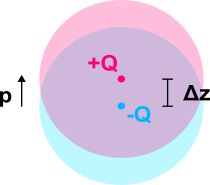
\includegraphics[width=0.38\textwidth]{images/chargepole} % Adjust width
\end{wrapfigure}

In questo modo il campo esterno alla sfera coincide con quello di un dipolo elettrico elementare con momento $\bold{p} = Q \Delta \bold{z}$ dove la carica 
\begin{equation*}
	Q = \mathcal{N} \frac{4}{3} \pi R^3 \varphi(r>R)	
\end{equation*}
e
\begin{equation*}
	\varphi = \frac{1}{4 \pi \varepsilon_0} \frac{\bold{p} \cdot \hat{u}_{r}}{r^2}
\end{equation*}
per legare il momento di dipolo elementare al vettore di polarizzazione aggiungiamo e sottraiamo dei termini
\begin{equation*}
	\bold{p} = \frac{4}{3}\pi R^2(\mathcal{N}q \Delta \bold{z}) = \frac{4}{3} \pi R^3 \bold{P}
\end{equation*}
e sostituendo all'interno dell'espressione del potenziale elettrostatico esterno della sfera otteniamo 
\begin{equation*}
	\varphi_{p} (r > R) = \frac{R^3}{3	\varepsilon_0} \frac{\bold{P} \cdot \hat{u}_{r}}{r^2} = \frac{R^3}{3 \varepsilon_0} \frac{P \cos\theta }{r^2}
\end{equation*} 
In questo modo possiamo calcolare il campo elettrico all'esterno 
\begin{equation*}
	\bold{E}(r>R) = - \nabla \varphi = \frac{R^3}{3 \varepsilon_0} \frac{P}{r^3} (2 \cos \theta \,\hat{u}_{r} + \sin \theta \, \hat{u}_{\theta})
\end{equation*}

\begin{wrapfigure}{l}{0.4\textwidth} % 'r' for right, 'l' for left
    \centering
    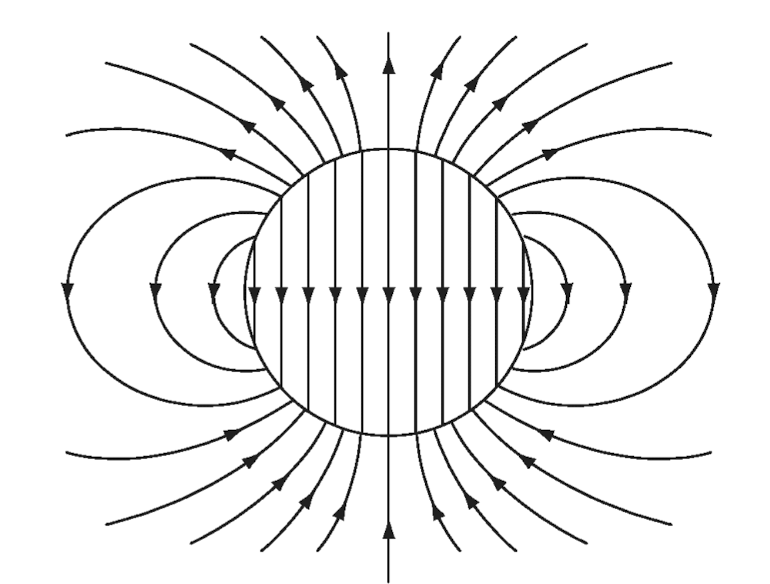
\includegraphics[width=0.38\textwidth]{images/dielpolarized} % Adjust width
\end{wrapfigure}
Il campo elettrico che troviamo esternamente alla sfera coincide con quello di un dipolo elettrico. Dai risultati precedenti conosciamo il potenziale sulla superficie della sfera
\begin{equation*}
	\varphi_{p}(r =R) = \frac{PR}{3 \varepsilon_0} \cos \theta = \frac{Pz}{3 \varepsilon_0}
\end{equation*}
che utilizziamo come condizione al contorno per l'equazione di Laplace $\nabla^2 \varphi = 0 $, siccome la soluzione del problema dell'elettrostatica esiste ed \`e unica, essendo $\varphi_{p}(r=R)$ una soluzione, il potenziale interno alla sfera \`e dato da 
\begin{equation*}
	\varphi(r < R) = \frac{Pz}{3 \varepsilon_0}
\end{equation*}
e quindi il campo elettrico interno alla sfera \`e dato da 
\begin{equation}
	\bold{E}_{p} = - \nabla \varphi = - \frac{\partial \varphi}{\partial z} \hat{u}_{z} = - \frac{\bold{P}}{3 \varepsilon_0}
\end{equation}
Sulla superficie \`e presenta una discontinuit\`a del campo data da
\begin{equation*}
	\Delta E_{r} = \frac{2P \cos \theta}{3 \varepsilon_0} - \left(- \frac{P \cos \theta}{3 \varepsilon_0}\right)=  \frac{P \cos \theta}{\varepsilon_0} =\frac{\sigma_{p}}{\varepsilon_0}
\end{equation*}
dovuta alla distribuzione di carica di polarizzazione superficiale.

Ipotizziamo ora che il mezzo sia lineare allora possiamo usare la relazione 
\begin{equation*}
	\bold{P} = \varepsilon_r \chi_{E} \bold{E}
\end{equation*}
siccome i campi costituenti $\bold{E}$ sono uniformi anch'esso lo \`e. Dall'equazione (7.33) possiamo definire il campo elettrico di polarizzazione rispetto a $\bold{P}$:
\begin{equation*}
	\bold{E}_{p} = - \frac{\chi_{E} }{3}\bold{E}
\end{equation*}
sostituendo nell'espressione $\bold{E} = \bold{E}_{s} + \bold{E}_{p}$ dopo alcuni conti si mette in relazione $\bold{E}_{s}$ con $\bold{P}$ e si risolve rispetto ad $\bold{E}$, in questo modo il campo \`e 
\begin{equation*}
	\bold{E} = \frac{3}{\varepsilon_r +2} \bold{E}_s
\end{equation*}
ovvero equiverso a $\bold{E}_{s}$, uniforme e $E < E_{s}$ in modulo. Mentre il vettore di polarizzazione \`e uniforme come ipotizzato
\begin{equation*}
	\bold{P} = \frac{3 \varepsilon_0(\varepsilon_r-1)}{\varepsilon_r +2}\bold{E}_{s}
\end{equation*}

\subsection{Altre strategie di risoluzione per problemi con i Dielettrici}
1) Principio di Sovrapposizione

\begin{wrapfigure}{l}{0.4\textwidth} % 'r' for right, 'l' for left
    \centering
    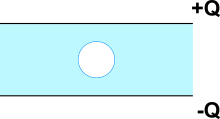
\includegraphics[width=0.38\textwidth]{images/voidplanar} % Adjust width
\end{wrapfigure}
Supponiamo di avere un dielettrico planare con un buco sferico nel suo centro. Per risolvere un problema di questo tipo possiamo ricorrere al principio di sovrapposizione, considerandolo come la differenza tra un sistema planare riempito di dielettrico con costante dielettrica $\varepsilon$, e un sistema dato da una sfera riempita di dielettrico con costante $- \varepsilon$.

Concettualmente si possono usare le medesime strategie usate nel caso elettrostatico.
\newline

\noindent 2) Metodo delle cariche immagine nei dielettrici

\begin{wrapfigure}{r}{0.4\textwidth} % 'r' for right, 'l' for left
    \centering
    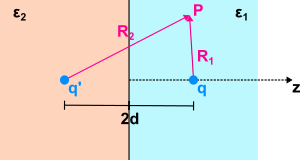
\includegraphics[width=0.38\textwidth]{images/polimage} % Adjust width
\end{wrapfigure}

Supponiamo di avere due mezzi dielettrici con costanti $\varepsilon_{1} \neq \varepsilon_{2}$ e che nella prima regione \`e posta una carica q ad una distanza $d$ dalla superficie di contatto tra i due materiali. Vogliamo determinare il campo elettrico in tutto il mezzo. 

Per farlo posizioniamo una carica immagine $q'$ simmetricamente alla prima nel secondo materiale. Per il campo nel punto $P$ devono valere le seguenti condizioni
\begin{equation*}
	\left \{ \begin{array}{l}
		\varepsilon_{1} E_{1,z}(z=0) = \varepsilon_{2}E_{2,z}(z=0) \\ \rule{0pt}{20pt}
		E_{1,x}(z=0) = E_{2,x}(z=0) \\ \rule{0pt}{20pt}
		E_{1,y}(z=0) = E_{2,y}(z=0)
	\end{array}\right.
\end{equation*}
(per calcolarle, vedere il paragrafo in cui si parla di due materiali comunicanti). Per $z>0$ il potenziale \`e dato da
\begin{equation*}
	\varphi_{1} = \frac{1}{4 \pi \varepsilon_1}\left(\frac{q}{R_1} + \frac{q'}{R_2}\right)
\end{equation*} 
dove 
\begin{equation*}
	R_{1} = \sqrt{(z-d)^2 + (x^2 + y^2)} \quad \text {e} \quad R_2 = \sqrt{(z+d)^2 + (x^2+y^2)}
\end{equation*}
In questo caso non possiamo risolvere il problema come fatto con il caso del conduttore, in cui la regione dove non \`e presenta carica \`e trascurabile, perch\`e in questo caso si ha del materiale dielettrico e quindi il potenziale non dipende da $q'$.

La soluzione pi\`u semplice \`e data da 
\begin{equation*}
	\varphi_{2} = \frac{1}{4 \pi \varepsilon_{2}} \frac{q''}{R_1}
\end{equation*}
per $z<0$. Dove la carica $q''$ \`e al posto della carica $q$, perch\`e se guardiamo il sistema dal lato di $\varepsilon_{2}$, si osserva una sorgente in nella stessa posizione di q, ma la carica non \`e la medesima in quanto il dielettrico $\varepsilon_{1}$ modifica l'intensit\`a del campo della sorgente puntiforme.

Posti $\rho^2 = x^2 + y^2$ nelle espressioni del raggio, passiamo alla geometria cilindrica e utilizzando le condizioni sul campo elettrico abbiamo che 
\begin{equation*}
	E_{\rho}(z = 0^+) = - \frac{\partial \varphi_{1}}{\partial \rho}\vert_{z=0} = - \frac{\partial \varphi_{2}}{\partial \rho}\vert_{z=0}=E(z=0^-)
\end{equation*}
sviluppando il calcolo di trovano le condizioni sulle cariche 
\begin{equation*}
	\left \{ \begin{array}{l}
		q'' = q - q' \\ \rule{0pt}{20pt}
		\varepsilon_{1}(q+q') = \varepsilon_2 q''
	\end{array}\right.
\end{equation*}

\section{Energia nei Dielettrici}

Per caricare un condensatore bisogna compiere un lavoro 
\begin{equation*}
	W = \frac{1}{2} C_0 V^2
\end{equation*}
Se il condensatore \`e riempito con un materiale dielettrico, mantenendo la tensione V = costante abbiamo che la capacit\`a viene incrementata di un fattore $\varepsilon_{r}$ rispetto a quella nel vuoto $C_0$:
\begin{equation*}
	C = \varepsilon_{r} C_0
\end{equation*} 
Per proporzionalit\`a diretta anche il lavoro deve essere incrementato di un medesimo fattore. Il motivo di questo incremento \`e semplice, dato che con la polarizzazione del mezzo si sviluppa della carica di polarizzazione sulla superficie del mezzo, parte del lavoro fornito viene convertito per alimentare questo processo; dunque per mantenere il potenziale costante V la batteria deve fornire una maggiore quanti\`a di carica libera.

Nel capitolo sull'elettrostatica abbiamo visto che l'energia immagazzinata da un qualsiasi campo elettrico \`e data da 
\begin{equation*}
	W = \frac{1}{2} \int_{V} \varepsilon_0 \bold{E}^2 d\nu
\end{equation*}
Nel caso in cui un condensatore \`e riempito di materiale dielettrico si ha che 
\begin{equation*}
	W = \frac{1}{2}\varepsilon_{0}\varepsilon_{r} \int_{V} \bold{E}^2 d\nu 
\end{equation*}
dato che $\bold{D} = \varepsilon_0 \bold{E} + \bold{P}$, se il mezzo lineare $\bold{P} = \varepsilon_0 \chi_{E} \bold{E}$ e quindi $\bold{D} = \varepsilon_{0}\varepsilon_{r}\bold{E}$, questo ci permette di esprimere l'energia come 
\begin{equation}
	W =  \frac{1}{2} \int_{V} \bold{D} \cdot \bold{E} d\nu
\end{equation}


